\chapter{引言}

\section{研究背景及意义}
% DL-based CV技术在医学图像上,对计算机辅助医疗应用的意义(辅助诊断、初级工作、快速准确)
医学图像的理解与分析是计算机辅助临床诊断的一种重要形式。近年来,随着深度学习技术的广泛应用与显著效果,医学图像领域的各种技术也快速发展,加快了智能医疗的进程。
医学图像的感知任务包括疾病诊断分类、异常特征检测、语义分割和实例分割等,它们可以作为先期诊断与辅助信息,在医学的不同的应用场景和不同阶段发挥重要作用,以实现自动化医学诊断或辅助医生判断。在国家医疗资源整体短缺的情况下,自动化智能化的医学图像感知系统可以极大地降低医生群体的工作量,显著提升处理效率,优化医疗流程,对整个医疗行业与社会具有深远意义。

% 作为一项基本课题,

% 图像的语义分割:任务描述,应用,数据标注的问题(标注不足,标签错误)
图像语义分割(Image Semantic Segmentation),是计算机视觉中的一个基本任务,旨在生成像素级的物体类别表征\citep{long2015fully,chen2017deeplab,ronneberger2015u,isensee2019automated}。而医学图像的语义分割,针对各种医学图像进行细粒度的感知和理解,如图~\ref{c1_fig1}所示,根据学习的医学知识生成重要的诊断论据。它对目标物体(比如器官、组织、肿瘤等)进行完整的识别,提供目标物体的形状或体积的关键信息,在计算机辅助医学中应用广泛。比如,对器官及所附肿瘤的分割结果,可以准确发现病灶和判断病型;血管的完整分割,能够作为手术操作的参考依据;肠道的分割建模,能够快速定位病灶。

    \begin{figure*}[t!]
        \centering 
        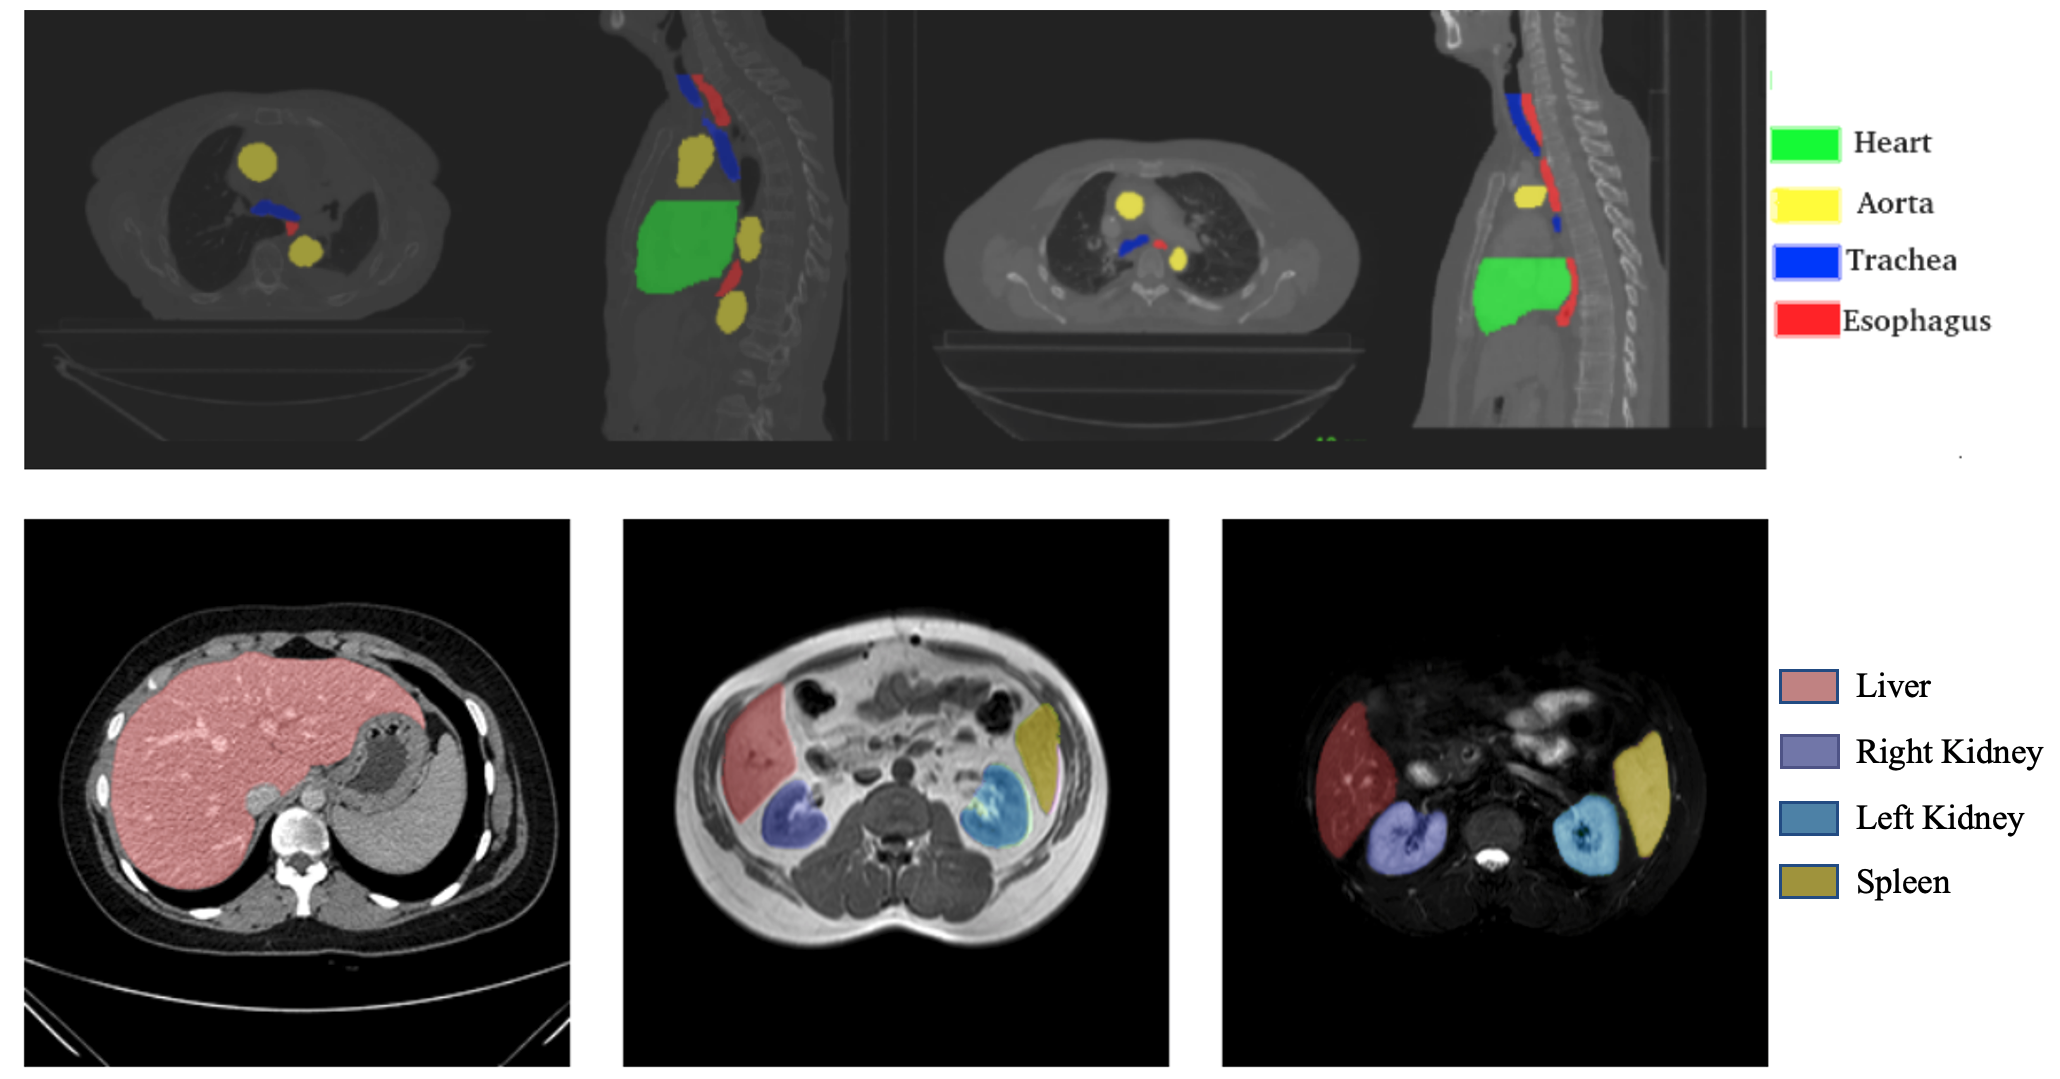
\includegraphics[width=1.0\textwidth]{img/c1/intro_1.png}
        \bicaption{医学图像中语义分割任务的例子:第一行是胸部 CT 图像\citep{lambert2020segthor},分割标注覆盖在原图像上,第二行是腹部的 CT、MR T1 和 MR T2 图像及其分割标注~\citep{kavur2021chaos}。}
        {Examples of medical image semantic segmentation. The first row shows images of thoracic organs, with an overlay of the manual segmentation, and the second row shows slices from abdominal organ in CT、MR T1 and MR T2 phases.
        DeepLab model training using image-level labels.}
        \label{c1_fig1}
    \end{figure*}

分割方法上,传统的图像语义分割依据图像的颜色、空间结构及纹理等特征来进行处理,包括聚类分割\citep{coates2012learning}、阈值分割\citep{ying2005fast}、决策树分割\citep{shotton2008semantic}、图割分割\citep{vicente2008graph}等。
近年来,随着深度学习技术的深入研究,特别是卷积神经网络(Convolutional Neural Network, CNN)在计算机视觉的广泛应用,语义分割技术迎来了新的发展。
通过深度神经网络的设计和优化算法,分割模型可以从大量的标注数据中自动学习提取丰富的高阶语义特征,在特征学习和表达能力上远优于前述的传统算法。模型基于提取的特征进行推理,从而预测图像的像素级类别标签。而随后的全卷积神经网络(Fully Convolutional Network, FCN)用卷积层替换传统 CNN 中的全连接层,通过端到端的全卷积网络设计,解决了输入图像的固定尺寸问题,极大提高了该任务的性能准确度与应用场景的广泛性。%接下来我们详述该任务的技术发展。

% 医学图像语义分割 背景
在图像语义分割任务中,全监督学习方法已经取得了很多进展,达到了较高的精度。这是其后研究弱监督语义分割的基础。
\citet{long2015fully}~针对传统神经网络要求固定尺寸的图像输入的问题,首次提出了接受任意尺寸输入的FCN,实现端对端的稠密预测。在此基础上,DeepLab~为了更精细的分割效果,在 CNN 的输出后使用全连接的条件随机场,以优化定位精度。更进一步,\citet{ronneberger2015u}~提出了一种编码器-解码器结构 U-Net,因其较好的泛化性能,这种结构被广泛应用在各种医学图像上。U-Net~的编码器采用一系列的卷积层和下采样操作,逐级提取语义信息,解码器则是一系列的卷积层和上采样操作,逐级恢复图像细节。U-Net兼顾了分割精度与效率。

上述工作都是在~2D~图像处理分割,而医学图像领域也有许多~3D~图像形式的分割任务。这些任务的每个输入样本,是连续的 2D 切片堆叠成的 3D 体积图像,输出目标也是 3D 分割掩膜。一种简单的思路是,输入端把 3D 任务拆解成 2D 任务,在每张 2D 切片上应用前述方法,输出时再将 2D 分割结果拼接成 3D 掩膜。但这样忽略了 3D 图像的整体性与内部联系,一些工作对端到端的 3D 图像分割方法进行了研究。3D~U-Net~\citep{cciccek20163d} 扩展了 U-Net,主要通过 3D 卷积单元替换 2D 卷积单元完成。这样整个 3D 图像可以直接输入进模型,输出端预测得到 3D 分割结果。随后,V-Net~\citep{milletari2016v} 则通过把残差连接引入卷积模块,用卷积层替换上采样和下采样的池化层,并提出 Dice 损失函数来克服类别不均衡,提高 3D 分割网络的特征表达能力与预测精度。
网络结构上的改进提高了分割性能,然而不同的任务常常需要不同的网络结构和训练策略。为了解决这一泛化问题,\citet{isensee2019automated}提出了 nnU-Net,这是一种鲁棒的自适应的分割框架,适用于大多数 2D 和 3D 图像,探索了自适应模型结构、前处理、训练和推理阶段的优化方案。nnU-Net 在多种图像的分割任务上都得到了最好的分割性能。

尽管全监督学习方法的进展迅速,高昂的标注成本却是实践应用的一个难题。训练基于深度学习的分割网络,通常需要一个较大的数据集,并且依赖大量像素级别的标注(能够准确地划分出物体边界)。然而在医学领域,由于缺乏有经验的标注者和物体边界的视觉模糊性,收集所需的高质量标签往往是困难的。并且,像素级的标注也非常耗时和昂贵。极高的标注成本一定程度阻碍了语义分割方法的应用效果,也限制了其应用场景的广度。因此,如何降低标注难度和成本是一个研究热点。

%过渡问题
不同于全监督学习,弱监督学习降低了所需标签的数量或质量,研究低成本下的学习方法。本文探索语义分割的弱监督学习,具体地,研究弱监督的两种形式:基于弱标签和基于噪声标签的学习。
基于弱标签的弱监督语义分割\citep{papandreou2015weakly,rajchl2016deepcut,cai2018accurate,ji2019scribble,kervadec2020bounding},放弃了要求较高的完整标签,采用弱标签方式,并探索基于其的高效分割方法。基于噪声标签的弱监督语义分割\citep{Zhu2019PickandLearnAQ,Xue2020CascadedRL,Zhang2020RobustMI},则研究如何充分利用噪声标签中的有效信息,并且避免其中的噪声干扰,以探索鲁棒的分割方法。
总结来说,弱监督语义分割是在有限条件的数据标注下,尽可能利用已有信息,并结合标签关系或分割特性等先验,提高分割效果,以接近基于完整准确标注方法(即全监督语义分割)的上限。
接下来我们分别详述基于弱标签和噪声标签的弱监督语义分割任务。

\subsection{基于弱标签的弱监督语义分割}
% 基于弱标签:问题转化、目标与实际意义
基于弱标签的弱监督语义分割,采用一些简单形式的标注方式,比如边界框、涂鸦式标签、点标签等,来进行图像分割模型的学习。图~\ref{c1_fig2}列出其中几种标签的示例,各自对应着不同的标注成本。
    \begin{figure*}[t!]
        \centering 
        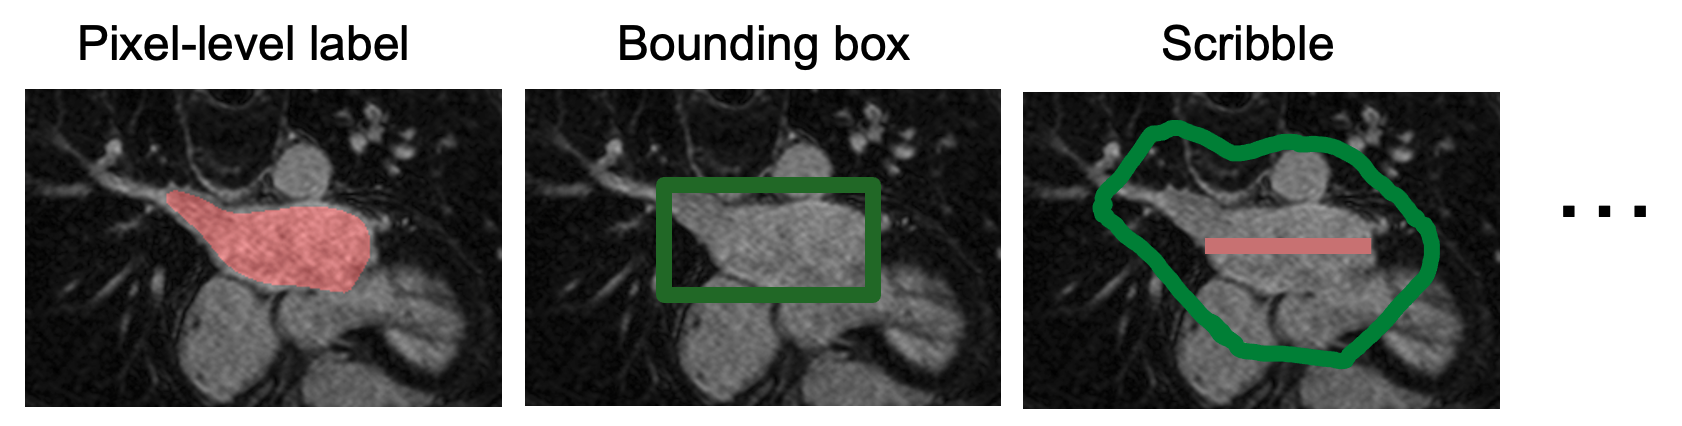
\includegraphics[width=1.0\textwidth]{img/c1/intro_2.png}
        \bicaption{医学图像上的弱标签示意图。从左到右依次是完整标签,边界框标签和涂鸦式标签。}
        {Different annotations on medical images. From left to right: groundtruth, bounding box and scribble.}
        \label{c1_fig2}
    \end{figure*}
由于弱标签提供的标签信息远少于全标注,语义信息有限,所以直接应用现有分割方法的输出精度较低。故而,如何充分利用弱标签来提高语义分割的效果,是一个重要问题。
在此方向的探索,实质上是采用各种技术,比如标签传播、图像结构或物体先验等,来弥补训练数据不足带来的效果下降。比如,人在识别目标物体时,即使缺少在细节的准确识别,仍可以根据物体的局部连续性或整体形状的先验,来准确地标出物体区域。在该问题的研究进展,能够广泛应用到各种训练数据不足的场景,对扩大深度学习技术的应用场景有重大意义。

近年来有很多工作对弱监督语义分割进行探索,并取得了相当的进展。
\citet{papandreou2015weakly} 探索使用边界框(bounding box)或图像级标签的标注方法,并提出了一种弱监督下的期望最大化(expectation maximization, EM)算法来训练语义分割模型。这种算法迭代地进行弱标注约束下的未知标签估计,和使用估计标签优化分割神经网络。EM 算法扩大了可训练数据的规模,且具有较好的性能,在后续的工作中被广泛使用。
\citet{lin2016scribblesup} 提出使用涂鸦(scribble)式标签进行图像标注,并且设计了一种算法来训练语义分割网络。该工作先设计一个图模型,以把涂鸦式标签传播到未标注像素上,然后利用传播后的标签学习一个全卷积网络,并反过来提供语义信息给图模型。这种结合图像结构建模的标签传播方法,提供了更多可信的训练标签。

% 弱标注的挑战
尽管这些工作探索了标签传播与优化训练的方法,但忽略了分割任务中的形状先验、结构先验等约束,容易生成不准确的物体形状。物体并不仅仅有局部视觉特征,也有整体的连续性与形状,充分考虑局部特征与整体特征的结合,对提高分割效果及算法的鲁棒性泛化性具有重要意义。
\citet{tang2018regularized} 采用基于正则化损失的弱监督方法,通过设计具有底层分割特性的正则项,来隐式地实现分割网络对底层特征的建模。这种正则项损失采用了马尔可夫随机场和条件随机场的形式。
\citet{kervadec2020bounding} 探索在边界框的弱标签上,在模型中引入一些全局约束条件,包括框内的紧致性先验和框外的全背景先验。这些约束条件被转化并结合进损失函数中进行优化。
这些方法利用底层或全局的先验,带来了一定程度的性能提高。但由于它们对先验的表达不足,或者依赖于特定的标注形式与超参数,有一定局限性。
%在弱监督分割中结合物体形状先验,仍然是一个需要探索的方向。


\subsection{基于噪声标签的弱监督语义分割}
% 基于噪声标签的语义分割:问题定义、目标和实际意义
基于噪声标签的弱监督语义分割,其训练数据中有一定比例的错误标签。由于医学图像本身的标注环境和难度,分割标签噪声是难以避免的,图~\ref{c1_fig3}给出一些标签易出错区域的示例。
噪声标签既包含有用的监督信息信号,也包含错误信息,直接使用会干扰神经网络的学习能力,降低模型的分割效果。这个任务的核心问题是如何识别并处理噪声标签,减少其对神经网络的影响。在现实的应用场景中,由于数据收集的复杂环境,噪声标签是很常见的,探索这一问题,有助于高效准确地用好这些标签。
    \begin{figure*}[t!]
        \centering 
        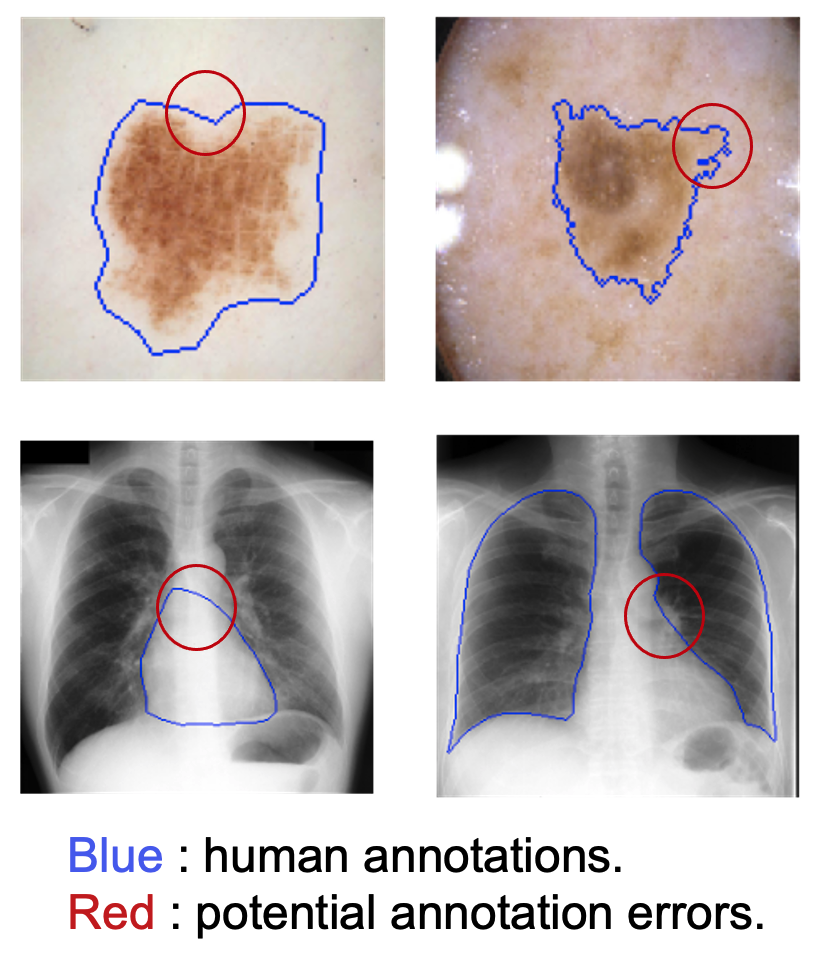
\includegraphics[width=0.7\textwidth]{img/c1/intro_3.png}
        \bicaption{医学图像上的噪声标签示意图。蓝色区域为人工标签,红色区域是可能的标签错误。}
        {Examples of noisy annotations of medical images. Blue curves show human annotations, while red curves point to potential errors.}
        \label{c1_fig3}
    \end{figure*}

% 有噪声标注 related
% 基于噪声标签的弱监督分割考虑另一种情况:标签中有一定比例的错误。错误标签如果不做处理,会直接损害神经网络的效果。
近来一些工作借鉴在分类任务的相似工作~\citep{arpit2017closer,Han2018CoteachingRT,Wei2020CombatingNL},对这一领域进行了探索。
\citet{Zhu2019PickandLearnAQ} 提出一种标签评估网络来自动评估标签质量,同时训练评估网络和分割网络,来自动重调整损失函数,以减轻错误标签对网络的负面影响。评估网络是基于损失值来筛选正确的训练样本,避免了噪声标签对训练的干扰。
但这种训练设计不够稳定,容易过拟合或欠收敛。其后,\citet{Zhang2020RobustMI} 设计了一种三网络共同学习的框架,用任两个网络来选择可信的样本给另一个网络,这种同步训练并相互教学的方式克服了单网络的缺点。
除了尽可能利用正确标签,改进错误标签能带来更多的训练信息。\citet{Xue2020CascadedRL} 结合了三网络相互教学的设计与标签改进的方法,以充分使用有效信息。其中的标签改进通过模型预测和后处理实现。
% 有噪声标注的挑战
上述工作相比于基线方法带来了很大的性能提升,然而,它们在分割方法上仍有不足,忽略了分割区域中的特征关系与空间结构,并且模型学习方法不够鲁棒。在这些方面的探索,依旧存在挑战性。


\section{本文研究内容}
本文根据分割任务的特点,分别探讨在弱监督语义分割中引入形状先验的作用,和基于图像底层特征表征的鲁棒学习方法。本节先是讨论基于弱标签和噪声标签的弱监督语义分割中现有的挑战与不足,根据方法的对比观察给出相应的思考。然后基于这些思考,提出我们的解决方法。对基于弱标签的语义分割,本文用自学习方法(self-taught learning)\footnote{本文的自学习方法具体是指在缺少真实形状标签的数据上,学习物体形状先验的方法。}捕捉物体的形状先验,以解决弱监督下分割形状的缺陷;对基于噪声标签的语义分割,本文采用超像素作为基本表征单元,并在其上进行模型更新和标签更新,以解决噪声标签的干扰问题。最后,我们总结了本文在这两个任务的主要贡献,表明了形状先验、结构特征等对于弱监督语义分割的重要性。

\subsection{基于弱标签的弱监督语义分割}
% 弱监督工作的局限,引入形状先验的意义
在基于弱标签的弱监督语义分割中,本文研究的重点是结合形状先验的分割方法。形状先验具有丰富的结构性特征,它既包含局部的连续性光滑性,也包含整体的结构统一性。本文目标是在弱监督语义分割中引入形状先验,来弥补仅仅依靠弱标签的训练信息的缺失。
过去的工作常常只把分割工作视为逐个像素的分类任务,而忽略其整体的几何结构。在分割任务中,局部视角下每个像素需要利用其视觉特征进行分类,但在全局视角下目标物体也有整体的形状。这种整体结构信息的建模,能够作为先验,克服局部的错误或缺失,引导模型产生更准确完整的分割结果。
特别是在医学图像领域,大多数物体都具有相对固定的形状,而同类物体通常具有一定程度的形状相似性。比如气管的管状结构及分叉,虽然不同个体的具体尺寸和位置不同,几何特征还是有较强的统一性。利用好形状先验,能够高效地解决弱标签带来的挑战,实现较低标注成本下的准确语义分割。

本文旨在探索用较少的标注成本达到较好的分割效果。我们主要关注三维体积图像的语义分割,现实世界中,很多医学图像都是三维形态的(比如CT、MRI等),而很多工作已经处理过二维图像,却对三维图像研究得较少,本文尝试弥补这方面的不足。
在弱监督的三维图像语义分割上,近来有很多工作采用把三维图像拆分成一组二维图像的处理策略。虽然这些基于二维的方法取得了不错的效果,但应用在三维图像时有以下局限。首先,它们只是将生成的二维掩膜堆叠在一起作为最终输出,因此往往会产生不准确的物体形状\citep{kervadec2019constrained,kervadec2020bounding}。此外,他们忽略了分割物体在三维空间中的连续性,并且无法利用连续的二维切片之间的标签相关性。由于这些限制与不足,在给定足够的三维样本和较小的片间间距条件下\citep{baumgartner2017exploration},二维方法往往比三维方法的表现要差。更进一步,现有的多数弱标签形式并不高效,无法为学习医学图像中的物体形状先验提供较好的指引。

本文提出了一种新的三维物体分割的弱监督学习策略,以解决上述的挑战。我们的主要想法包括两个方面。首先,本文提出了一种自学习方法,通过使用弱标签来学习形状表征和样本增强的方法,来捕捉目标物体类别的三维形状先验。随后,这种学习到的形状先验与分割模型结合,参与模型的训练和推理过程。此外,本文提出了一种稀疏的弱标注方案,可以减少低效的标注,更好地利用物体标签的空间连续性,并且促进形状上下文的学习。

为了实现这一目标,本文设计了一个由两个主要模块组成的深度神经网络:一个是标准的语义分割网络,它从三维输入图像中产生一个初始的三维分割掩膜;另一个是形状去噪网络,它对初始分割掩膜进行改进并输出一个最终的三维分割。为了训练深度网络,我们首先引入一种稀疏的弱标注方案,该方案只需标注三维数据的一个子集(即一部分二维图像切片),同时对每张二维图像,我们设计了一种混合式弱标签,它结合了前景涂鸦和目标物体的一个宽松边界框。给定这样的弱标注形式,我们为网络模型设计了一个迭代学习框架,交替进行像素级标签生成和网络参数更新。

具体地,本文首先使用弱标签训练语义分割模块,来初始化分割网络模型,该模块为训练数据预测生成了初始分割掩膜。然后利用这些初始掩膜,我们用自学习方法来学习形状去噪模块。为此,文中把形状去噪模块实例化为一个去噪自动编码器(denoising autoencoder)\citep{vincent2010stacked,Sundermeyer_2018_ECCV},并选择具有最高置信度的掩膜预测作为目标形状来训练。为了模拟生成对应目标形状的噪声掩膜输入,本文根据初始掩膜预测中的经验错误模式,对目标形状应用了几种噪声增强方案。在模型初始化之后,本文的学习策略迭代地执行两步更新:像素级的伪标签生成,和神经网络学习。对于标签生成,我们采用一个不确定性过滤机制融合语义分割模块和形状去噪模块的预测输出,这使得可以利用学习到的形状先验来提高标签质量。在网络学习中,我们冻结了形状去噪网络,并在原始弱标签和生成标签的双重监督下更新语义分割网络。

我们在两个公开的医学图像数据集上评估所提的方法,这两个数据集的目标器官具有不同的形状特征,分别是SegTHOR挑战赛\citep{trullo2019multiorgan}中的气管和Promise12挑战赛\citep{Litjens2014EvaluationOP}中的前列腺。实验结果表明,在多种稀疏弱标注的设定下,本文的方法都优于以前的方法。不仅如此,在少量的标注条件下(10\%的二维切片标注),其他现有方法的效果大幅下降,而我们取得了鲁棒准确的结果。

\subsection{基于噪声标签的弱监督语义分割}
% Noisy工作的局限,引入结构先验与空间关系的意义
在基于噪声标签的弱监督语义分割中,本文探索在分割任务中利用像素间相关性和空间先验等特性,并且设计新的鲁棒学习方法。
过去的许多工作,忽略了分割任务的特性,把每个像素看做独立同分布的样本来建模。为了克服这样的局限性,本文考虑使用更灵活的表征和训练策略,来捕捉分割图像的底层特征与性质。比如在标签选择中提供更可靠的置信度,尽可能挖掘物体边缘的有效信息或难样本,从而更准确地使用和处理噪声标签。

本文要解决的重点问题是防止分割网络过拟合到噪声标签的模式上。本部分沿袭现有工作的设定,研究二维图像上的鲁棒学习方法。
%由于该方向刚起步,现有工作较少,本部分沿袭之前工作的设定,研究二维图像上的鲁棒学习方法。
目前已经有一些工作研究使用噪声标签来训练分割网络,大体上可以分为两类。第一类方法以整张图像为基本单位,把每个图像样本的标签都视为正确或错误的,然后在训练过程中迭代地选择或重加权图像样本\citep{Zhu2019PickandLearnAQ,Xue2020CascadedRL}。具体来说,\citet{Zhu2019PickandLearnAQ}通过同时训练一个标签评估网络和一个分割网络,隐式地对图像的损失函数进行重新加权,而\citet{Xue2020CascadedRL}通过将协同教学(Co-teaching~\cite{Han2018CoteachingRT})\footnote{协同教学(co-teaching)与协同训练(co-training)的区别如下:协同教学是基于噪声标签的训练方法,利用不同网络的相互教学来降低噪声影响。而协同训练是半监督学习中的方法,使用有标注数据中不同视图的特征来训练模型,并扩大训练集的标签规模。} 方案扩展到一个三网络学习框架,显式地选择一部分图像进行训练。然而,这种图像级的加权策略在严重的噪声设定下表现较差,因为它们无法充分利用每张图像中具有正确标签的像素。为了解决这一局限性,第二类训练方法将分割视为像素级分类任务~\citep{Zhang2020CharacterizingLE,Zhang2020RobustMI},在训练中,根据近期的鲁棒的分类器学习策略来进行像素级别的样本选择或标签改进,比如置信度学习技术~\citep{Zhang2020CharacterizingLE}或三网络协同教学方法\citep{Zhang2020RobustMI}。尽管他们更充分地利用了标签,但基于像素的方法忽略了图像分割中的像素相关性和空间先验关系,因此容易在目标物体边界周围产生噪声预测,降低分割效果。

本文为图像语义分割提出了一种新的鲁棒的学习策略,目标是利用好图像的结构先验和像素标签的相关性。为此,我们采用了图像的超像素表征,并设计了一个迭代学习方案,这个方案结合了分割网络的噪声感知训练过程和噪声标签改进过程,两者都由超像素引导。这种结合使我们能够更好地利用分割标签的结构约束来进行模型学习,从而有效地减轻噪声标签的影响。我们注意到,虽然超像素在最近的工作中也被采用\citep{li2019supervised},但他们只在标签改进中使用,而忽略了训练阶段对噪声标签的处理。

具体来说,在每次迭代中,本文首先使用选定的具有较小损失值的超像素子集来同时训练一组孪生网络,这遵循了多视图学习框架\citep{Han2018CoteachingRT,Wei2020CombatingNL}。正如在协同教学方法中一样,这种多视图学习策略通过利用孪生网络的预测来约束网络训练。文中将每个超像素作为一个数据样本进行选择,因此能够在网络训练中引入底层空间特征并提供较好的物体边界引导。为了避免模型过拟合到噪声标签,我们根据超像素的损失值统计,为联合学习设计了一个自动停止的标准。在网络训练之后,我们使用网络预测来估计超像素标签的置信度,并对置信度最低的标签子集进行修正。这种标签修正方法能够在后续模型训练中提高标签质量,进而提升训练效果。网络和标签更新会互相迭代,直到标签修正无法再取得进一步的改善。

本文所提出的方法在两个公开的基准数据集上进行了评估,包括 ISIC 皮肤病变数据集\citep{Gutman2018SkinLA}和 JSRT 胸部 X 射线数据集\citep{Ginneken2006SegmentationOA,Shiraishi2000DevelopmentOA},并测试了大量的噪声水平设定。在一系列的噪音水平的设定下,实验结果表明我们的方法全都超过以往的工作,并表现出优越的训练鲁棒性。

\subsection{主要贡献}
本文从降低分割任务中所需标注成本入手,分别在基于弱标签和噪声标签的弱监督语义分割两方面做出了贡献。

在基于弱标签的弱监督语义分割任务中,我们的主要贡献有三个方面:
\begin{enumerate}
\item 本文设计了一种形状感知的弱监督三维图像分割方法,它将自学习得到的形状去噪网络与分割网络结合。本文还设计了一种迭代方法来进行有效的神经网络学习。
\item 本文为三维图像分割提出了一种新的稀疏的混合式弱标注策略。
\item 在相同的标注成本下,本文的方法在多种标注密度的设定下都实现了最好的性能。
\end{enumerate}


基于噪声标签的弱监督语义分割任务中,我们的贡献分以下三方面:
\begin{enumerate}
    \item 在基于噪声标签的语义分割中,本文引入了超像素表征,以通过利用图像结构先验来增强模型的鲁棒性。
    \item 本文设计了一种包括模型更新和标签改进的迭代学习策略,以充分利用训练数据并逐步提高分割质量。
    \item 与现有最好的方法相比,本文的方法在一系列噪声水平设定下,都实现了更好的性能和鲁棒性。
\end{enumerate}

\section{本文结构}
本节介绍全文的行文组织结构。

第一章为引言部分,主要介绍医学图像语义分割的标注挑战的背景,并引出基于弱标签和噪声标签的弱监督语义分割这两个任务,随后介绍本文在这两个方向的主要研究内容。

第二章为相关工作部分,我们对基于弱标签的语义分割、自学习方法、降噪自编码器、基于噪声标签的语义分割等方向的现有工作进行总结。

第三章开始详述第一个任务的内容,即结合形状先验的弱监督语义分割。本部分我们先形式化描述基于弱标签的分割任务,然后引出所提出的结合形状先验的分割模型。再后介绍我们提出的稀疏的弱标注策略、模型训练过程,最后是详尽的实验来对比验证模型的效果。

第四章是第二个任务的内容,即基于噪声标签的语义分割。这部分与上一章结构相似,依次介绍了该任务的形式化描述,模型设计,超像素表征,迭代的模型学习方法,实验对比与分析等部分。

第五章是全文的总结与展望。该部分总结了本文在弱监督语义分割的两个方向的方法设计与贡献,并探讨了该领域未来的研究趋势。